\chapter{Formal Definition}
\label{chap:definition}

\section{Requirements}
\label{sec:requirements}
The Graphalytics benchmark is the result of a number of design choices.

\begin{itemize}
\item[\textbf{(R1)}] \textbf{Target platforms and systems:} benchmarks must support any graph analysis platform operating on any underlying hardware system. For platforms, we do not distinguish between programming models and support any model. For systems, we target the following environments: 
%distributed systems, multi-core single-node systems, many-core GPU systems, hybrid CPU-GPU systems, and distributed hybrid systems. 
multi-core and many-core single-node systems, systems with accelerators (GPUs, FPGAs, ASICs), hybrid systems, and distributed systems that possibly combine several of the previous types of environments.
Without R1, a benchmark could not service a diverse industrial following.

\item[\textbf{(R2)}] \textbf{Diverse, representative benchmark elements:} data model and workload selection must be representative and have a good coverage of real-world practice. In particular, the workload selection must include datasets and algorithms which cover known system bottlenecks and be representative in the current and near-future practice. Without representativeness, a benchmark could bias work on platforms and systems towards goals that are simply not useful for improving current practice. Without coverage, a benchmark could push the community into pursuing cases that are currently interesting for industry, but not address what could become impassable bottlenecks in the near-future.

\item[\textbf{(R3)}] \textbf{Diverse, representative process:} the set of experiments conducted by the benchmark automatically must be broad, covering the main bottlenecks of the target systems. \futureinversion{2.0}{In particular, the target systems are known to raise various scalability issues, and also, because of deployment in real-world clusters, be prone to various kinds of failures, exhibit performance variability, and overall have various robustness problems.} The process must also include validation of results, thus making sure the processing is done correctly. Without R3, a benchmark could test very few of the diverse capabilities of the target platforms and systems, and benchmarking results could not be trusted.

\item[\textbf{(R4)}] \textbf{Include renewal process:} unlike many other benchmarks, benchmarks in the area of graph processing must include a renewal process, that is, not only a mechanism to scale up or otherwise change the workload to keep up with increasing more powerful systems, but also a process to automatically configure the mechanism, and a way to characterize the reasonable characteristics of the workload for an average platform running on an average system. Without R4, a benchmark could become less relevant for the systems of the future.

\item[\textbf{(R5)}] \textbf{Modern software engineering:} benchmarks must include a modern software architecture and run a modern software-engineering process. The Graphalytics benchmark is provided with an extensive benchmarking suite that allows users to easily add new platforms and systems to test. This makes it possible for practitioners to easily access the benchmarks and compare their platforms and systems against those of others. Without R5, a benchmark could easily become unmaintainable or unusable.
\end{itemize}


\section{Data}
The Graphalytics benchmark operates on a single type of dataset: graphs. This section provides the definition of a graph, the definition of the representation used by Graphalytics for its input and output data, and the datasets used for the benchmarks.

\subsection{Definition}
Graphalytics does not impose any requirements on the semantics of the graph. The benchmark uses a typical data model for graphs. A graph consists of a collection of \emph{vertices} (nodes) which are linked by \emph{edges} (relationships).  Each vertex is assigned a unique identifier represented as a signed 64-bit integer, i.e., between $-2^{63}$ and $2^{63}-1$. Vertex identifiers do not necessarily start at zero, nor are the identifiers necessarily consecutive. Edges are represented as pairs of vertex identifiers. Graphalytics supports both \emph{directed} graphs (i.e., edges are unidirectional) and \emph{undirected} graphs (i.e., edges are bidirectional). Every edge is unique and connects two distinct vertices. This implies that self-loops (i.e., vertices having edges to themselves) and multi-edges (i.e., multiple edges between a pair of vertices) are not allowed. In the case of undirected graphs, for every pair of vertices $u$ and $v$, the edges $(u,v)$ and $(v,u)$ are considered to be identical.

Vertices and edges can have properties which can be used to store meta-data such as weights, timestamps, labels, costs, or durations. Currently, Graphalytics supports three types of properties: \emph{integers}, \emph{floating-point numbers}, and \emph{booleans}. All floating-point numbers must be internally stored and handled in 64-bit double-precision IEEE 754 format. We explicitly do not allow the single precision format, as this can speedup computation and presents an unfair advantage. The current specification of Graphalytics does not use integer or boolean properties.


\subsection{Representation}\label{sec:data:representation}
In Graphalytics, the file format used to represent the graphs is the ``Edge/Vertex-List with Properties'' (\emph{EVLP}) format for graphs. The format consists of two text files: a vertex-file containing the vertices (with optional properties) and an edge-list containing the edges (with optional properties). Both files are plain text (ASCII) and consist of a sequence of lines.

For the vertex files, each line contains exactly one vertex identifier. The vertex identifiers are sorted in ascending order to facilitate easy conversion to other formats. For the edge files, each line contains two vertex identifiers separated by a space. The edges are sorted in lexicographical order based on the two vertices. For directed graphs, the source vertex is listed first. For undirected graphs, the smallest identifier of the two vertices is listed first and each edge is only listed once in one direction.

Vertices and edges can have optional properties. These values of these properties are listed in the vertex/edge files after each vertex/edge and are separated by spaces. The interpretation of these properties is not provided by the files.

\begin{figure}[t!]
\centering
\begin{subfigure}{0.3\textwidth}
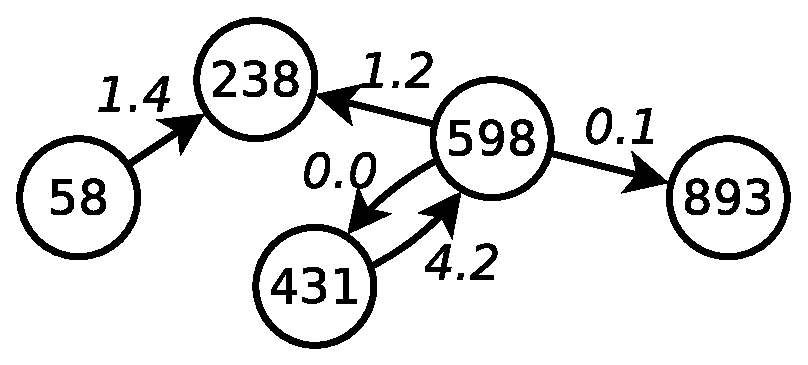
\includegraphics[width=0.9\textwidth]{figures/example_evlp}
%\caption{Graph}
\end{subfigure}
\begin{subfigure}{0.3\textwidth}
\begin{Verbatim}[frame=single]
58 
238
431
598
893
\end{Verbatim}
%\caption{Vertex file}
\end{subfigure}
\begin{subfigure}{0.3\textwidth}
\begin{Verbatim}[frame=single]
58 238 1.4
431 598 4.2
598 238 1.2
598 431 0.0
598 893 0.1
\end{Verbatim}
%\caption{Edge file}
\end{subfigure}
\newline
\newline
\begin{subfigure}{0.3\textwidth}
  \centering
  (a) Graph
\end{subfigure}
\begin{subfigure}{0.3\textwidth}
  \centering
  (b) Vertex file
\end{subfigure}
\begin{subfigure}{0.3\textwidth}
  \centering
  (c) Edge file
\end{subfigure}

\caption{Example of directed weighted graph in EVLP format.}
\label{fig:definition_example_evlp}
\end{figure}

Figure~\ref{fig:definition_example_evlp} shows an example of the EVLP format for a small directed weighted graph consisting of 5 vertices and 5 directed edges.


\subsection{Size and Scale}
\label{sec:definition_scale}

Graphalytics includes both graphs from real-world applications and synthetic graphs which are created using graph generators. Graphalytics uses a broad range of graphs with a large variety in domain, size, density, and other characteristics. To facilitate performance comparison across datasets, the \emph{scale} of a graph is derived from the number of vertices ($n$) and the number of edges ($m$). Formally, the scale of a graph is defined by calculating the sum $n + m$, taking the logarithm of this value in base 10, and truncating the result to one decimal place. Formally, this can be written as follows:
%
\begin{equation}
\textit{Scale}(n, m) = \lfloor 10 \log_{10}(n + m) \rfloor / 10
\end{equation}
%
The scale of a graph gives users an intuition of what the size of graph means in practice. Scales are grouped into classes spanning 0.5 \emph{scale units} and these classes are labeled using familiar system of ``T-shirt sizes'': small (S), medium (M), and large (L), with extra (X) prepended for extremes scales. The reference point is class L, which is defined by the Graphalytics team as the largest class such that the BFS algorithm completes within an hour on any graph from that scale using a state-of-the-art graph analysis platform and a single commodity machine. Table~\ref{tab:definition_scales} summarizes the classes used in Graphalytics.


\begin{table}
\caption{Mapping of dataset scales (``T-shirt sizes'') in Graphalytics.}
\label{tab:definition_scales}

\centering
\begin{tabular}{|l||c|}
\hline
\textbf{Label} & \textbf{Scales} \\ %& \textbf{Number of vertices and edges} \\
\hline \hline
2XS & $6.5 - 6.9$ %& $3.2 \times 10^{6} - 10^{7} $ 
\\ \hline
XS & $7.0 - 7.4$ %& $10^{7} - 3.2  \times 10^{7}$ 
\\ \hline
S & $7.5-7.9$ %& $3.2 \times 10^{7} - 10^{8} $
 \\ \hline
M & $8.0 - 8.4$ %& $10^{8} - 3.2 \times 10^{8}$ 
\\ \hline
L & $8.5 - 8.9$ %& $3.2 \times 10^{8} - 10^{9} $
\\ \hline
XL & $9.0 - 9.4$ %& $ 10^{9} - 3.2 \times 10^{9}$
 \\ \hline
2XL & $9.5 - 9.9$ %& $3.2 \times 10^{9} - 10^{10}$  
\\ \hline
3XL & $10.0 - 10.4$ %& 10^{10} - 3.2 \times 10^{10}$
\\ \hline
\end{tabular}
\end{table}


\subsection{Datasets}\label{sec:definition_datasets}
Graphalytics uses both graphs from real-world applications and synthetic graphs which are generated using data generators, the selection of which spans a variety of sizes and densities.

\paragraph{Real-world Datasets} By including real-world graphs from a variety of domains, Graphalytics covers users from different communities, including graphs from the knowledge, gaming, and social network domains.  Table~\ref{tab:real-datasets} lists the real-world datasets used by the Graphalytics benchmark.

\begin{table}[h]
\caption{Real-world datasets used by Graphalytics.}
\label{tab:real-datasets}
\centering
\begin{tabular}{|l|l|r|r|r|l|}
\hline
\textbf{ID} & \textbf{Name} & \textbf{$n$} & \textbf{$m$} & \textbf{Scale} & \textbf{Domain} \\
\hline
R1(2XS) & wiki-talk~\cite{snapnets} & 2.39\,M & 5.02\,M & 6.9 & Knowledge \\
\hline
R2(XS) & kgs~\cite{DBLP:conf/netgames/GuoI12} & 0.83\,M & 17.9\,M & 7.3 & Gaming \\
\hline
R3(XS) & cit-patents~\cite{snapnets} & 3.77\,M & 16.5\,M & 7.3 & Knowledge \\
\hline
R4(S) & dota-league~\cite{DBLP:conf/netgames/GuoI12} & 0.06\,M & 50.9\,M & 7.7 & Gaming \\
\hline
R5(XL) & com-friendster~\cite{snapnets} & 65.6\,M & 1.81\,B & 9.3 & Social \\
\hline
R6(XL) & twitter\_mpi~\cite{DBLP:conf/icwsm/ChaHBG10} & 52.6\,M & 1.97\,B & 9.3 & Social \\
\hline
\end{tabular}
\end{table}


\futureinversion{2.0}{Renew the graph selection process for real-world graphs, using new graph data archive, for example, with suggestion from Mihai....}



\paragraph{Synthetic Datasets} Besides real-world datasets, Graphalytics adopts two commonly used generators that generate two types of graphs: power-law graphs from the \textbf{Graph500} generator~\cite{chakrabarti2004, murphy2010} and social network graphs from \textbf{LDBC Datagen}~\cite{DBLP:conf/sigmod/ErlingALCGPPB15}. Tables~\ref{tab:graph500-datasets} and \ref{tab:datagen-datasets} list the Graph500 datasets and the Datagen datasets.



\begin{table}[h]
\caption{Synthetic Graph500 datasets used by Graphalytics.}
\label{tab:graph500-datasets}
\centering
\begin{tabular}{|l|l|r|r|r|}
	\hline
	\textbf{ID} & \textbf{Name} &   $n$ &    $m$ & \textbf{Scale} \\ \hline\hline
	G22(S)      & Graph500-22   &  2.4M &  64.2M &            7.8 \\ \hline
	G23(M)      & Graph500-23   &  4.6M & 129.3M &            8.1 \\ \hline
	G24(M)      & Graph500-24   &  8.9M & 260.4M &            8.4 \\ \hline
	G25(L)      & Graph500-25   & 17.0M & 523.6M &            8.7 \\ \hline
	G26(XL)     & Graph500-26   & 32.8M &   1.1B &            9.0 \\ \hline
	G27(XL)     & Graph500-27   & 65.6M &   2.1B &            9.3 \\ \hline
	G28(2XL)    & Graph500-28   &  121M &   4.2B &            9.6 \\ \hline
	G29(2XL)    & Graph500-29   &  233M &   8.5B &            9.9 \\ \hline
	G30(3XL)    & Graph500-30   &  448M &  17.0B &           10.2 \\ \hline
\end{tabular}
\end{table}


\begin{table}[t!]
\caption{Synthetic Datagen datasets used by Graphalytics.}
\label{tab:datagen-datasets}
\centering
\begin{tabular}{|l|l|r|r|r|}
\hline
\textbf{ID} & \textbf{Name} & $n$ & $m$ & \textbf{Scale} \\
\hline \hline
D7.5(S) & Datagen-7.5-fb & 0.6M & 34.2M & 7.5 \\ \hline
D7.6(S) & Datagen-7.6-fb & 0.8M & 42.2M & 7.6 \\ \hline
D7.7(S) & Datagen-7.7-zf & 13.2M & 32.8M & 7.6 \\ \hline
D7.8(S) & Datagen-7.8-zf & 16.5M & 41.0M & 7.7 \\ \hline
D7.9(S) & Datagen-7.9-fb & 1.4M & 85.7M & 7.9 \\ \hline
D8.0(M) & Datagen-8.0-fb & 1.7M & 107.5M & 8.0 \\ \hline
D8.1(M) & Datagen-8.1-fb & 2.1M & 134.3M & 8.1 \\ \hline
D8.2(M) & Datagen-8.2-zf & 43.7M & 106.4M & 8.1 \\ \hline
D8.3(M) & Datagen-8.3-zf & 53.5M & 130.6M & 8.2 \\ \hline
D8.4(M) & Datagen-8.4-fb & 3.8M & 269.5M & 8.4 \\ \hline
D8.5(L) & Datagen-8.5-fb & 4.6M & 332.0M & 8.5 \\ \hline
D8.6(L) & Datagen-8.6-fb & 5.7M & 422.0M & 8.6 \\ \hline
D8.7(L) & Datagen-8.7-zf & 145.1M & 340.2M & 8.6 \\ \hline
D8.8(L) & Datagen-8.8-zf & 168.3M & 413.4M & 8.7 \\ \hline
D8.9(L) & Datagen-8.9-fb & 10.6M & 848.7M & 8.9 \\ \hline
D9.0(XL) & Datagen-9.0-fb & 12.9M & 1.0B & 9.0 \\ \hline
D9.1(XL) & Datagen-9.1-fb & 16.1M & 1.3B & 9.1 \\ \hline
D9.2(XL) & Datagen-9.2-zf & 434.9M & 1.0B & 9.1 \\ \hline
D9.3(XL) & Datagen-9.3-zf & 555.3M & 13.1B & 9.2 \\ \hline
D9.4(XL) & Datagen-9.4-fb & 29.3M & 2.6B & 9.4 \\ \hline
D-3k(XL) & Datagen-sf3k-fb & 33.5M & 2.9B & 9.4 \\ \hline
D-10k(2XL) & Datagen-sf10k-fb & 100.2M & 9.4B & 9.9 \\ \hline
\end{tabular}
\end{table}



\section{Algorithms}
\label{sec:definition_algorithms}

The Graphalytics benchmark consists of six algorithms (also known as \emph{kernels}~\cite{DBLP:conf/hipc/BaderM05}) which need to be executed on the different datasets: five algorithms for unweighted graphs and one algorithm for weighted graphs. These algorithms have been selected based on the results of multiple surveys and expert advice from the participants of the LDBC Technical User Community (TUC) meeting.

Each workload of Graphalytics consists of executing a single algorithm on a single dataset. Below, abstract descriptions are provided for the six algorithms; pseudo-code is given in Appendix~\ref{chap:algorithms}. Furthermore, a link to the reference implementation is presented in \sref{sec:instructions:drivers}. However, Graphalytics does not impose any constraint on the implementation of algorithms. Any implementation is allowed, as long as its correctness can be validated by comparing its output to correct reference output (Section~\ref{sec:definitions_validation}). 

In the following sections, a graph $G$ consists of a set of vertices $V$ and a set of edges $E$. For undirected graphs, each edge is bidirectional, so if $(u,v)\in E$ then $(v,u)\in E$. Each vertex $v$ has a set of outgoing neighbors
$N_\mathrm{out}(v) = \{u \in V | (v, u) \in E \}$, a set of incoming neighbors
$N_\mathrm{in}(v)  = \{u \in V | (u, v) \in E \}$, and a set of all neighbors
$N(v) = N_\mathrm{in}(v) \cup N_\mathrm{out}(u)$.
Note that for undirected graphs, each edge is bidirectional so we have $N_\mathrm{in}(v) = N_\mathrm{out}(v) = N(v)$.


\subsection{Breadth-First Search (BFS)}
\label{sec:bfs}
\emph{Breadth-First Search} is a traversal algorithm that labels each vertex of a graph with the length (or \emph{depth}) of the shortest path from a given source vertex (\emph{root}) to this vertex. The root has depth $0$, its outgoing neighbors have depth $1$, their outgoing neighbors have depth $2$, etc. Unreachable vertices should be given the special value of $-1$. Example graphs are shown in \autoref{fig:bfs_example}.


\subsection{PageRank (PR)}
\label{sec:pr}
\emph{PageRank} is an iterative algorithm that assigns to each vertex a ranking value. The algorithm was originally used by Google Search to rank websites in their search results~\cite{page1999pagerank}. Let $\textit{PR}_i(v)$ be the PageRank value of vertex $v$ after iteration $i$. Initially, each vertex $v$ is assigned the same value such that the sum of all vertex values is $1$.
%
\begin{equation}
\textit{PR}_0(v) = \frac{1}{|V|}
\end{equation}
%
After iteration $i$, each vertex pushes its PageRank over its outgoing edges to its neighbors. The PageRank for each vertex is updated according to the following rule:
%
\begin{equation}
\textit{PR}_i(v) =
  \underbrace{\frac{1-d}{|V|}}_\textit{teleport} +
  \underbrace{d \cdot \sum_{u \in N_\mathrm{in}(v)} \frac{\textit{PR}_{i - 1}(u)}{|N_\mathrm{out}(u)|}}_\textit{importance} +
  \underbrace{\frac{d}{|V|} \cdot \sum_{w \in D} \textit{PR}_{i - 1}(w)}_\textit{redistributed from dangling}
\end{equation}
%
Notation: $d \in [0,1]$ is the \emph{damping factor} and $D = \big\{w \in V \ \big| \ |N_\mathrm{out}(w)| = 0 \big\}$ is the set of \emph{dangling vertices}, i.e., vertices having no outgoing edges.
Dangling vertices have nowhere to push their PageRank to, so the total sum of the PageRanks for the dangling vertices is evenly distributed over all vertices~\cite{DBLP:conf/www/EironMT04}.
When computing the $\textit{importance}$ value, we consider $\frac{\textit{PR}_{i}(u)}{|N_\mathrm{out}(u)|}$ to be $0$ for dangling vertices. 

The PageRank algorithm should continue for a fixed number of iterations. The floating-point values must be handled as 64-bit double-precision IEEE 754 floating-point numbers. 


\subsection{Weakly Connected Components (WCC)}
\label{sec:wcc}
This algorithm finds the \emph{Weakly Connected Components} of a graph and assigns each vertex a unique label that indicates which component it belongs to. Two vertices belong to the same component, and thus have the same label, if there exists a path between these vertices along the edges of the graph. For directed graphs, it is allowed to travel over the reverse direction of an edge, i.e., the graph is interpreted as if it is undirected.
Example graphs are shown in \autoref{fig:wcc_example}.

\subsection{Community Detection using Label Propagation (CDLP)}
\label{sec:cdlp}
The \emph{community detection} algorithm in Graphalytics uses \emph{label propagation} (CDLP) and is based on the algorithm proposed by Raghavan et al.~\cite{raghavan2007near}. The algorithm assigns each vertex a label, indicating its community, and these labels are iteratively updated where each vertex is assigned a new label based on the frequency of the labels of its neighbors. The original algorithm has been adapted to be both deterministic and parallel, thus enabling output validation and parallel execution.

Let $L_i(v)$ be the label of vertex $v$ after iteration $i$. Initially, each vertex $v$ is assigned a unique label which matches its identifier.
%
\begin{equation}
L_0(v) = v
\end{equation}
%
In iteration $i$, each vertex $v$ determines the frequency of the labels of its incoming and outgoing neighbors and selects the label which is most common.  If the graph is directed and a neighbor is reachable via both an incoming and outgoing edge, its label will be counted twice. In case there are multiple labels with the maximum frequency, the smallest label is chosen. In case a vertex has no neighbors, it retains its current label. This rule can be written as follows:
%
\begin{equation}
L_i(v) = \min \left( \underset{l}{\mathrm{arg\,max}} \Bigg[ \Big|\{ u \in N_\mathrm{in}(v)~|~L_{i-1}(u) = l \}\Big| + \Big|\{ u \in N_\mathrm{out}(v)~|~L_{i-1}(u) = l \}\Big| \Bigg] \right)
\end{equation}

Example graphs are shown in \autoref{fig:cdlp_example}.

\subsection{Local Clustering Coefficient (LCC)}
\label{sec:lcc}
The \emph{Local Clustering Coefficient} algorithm determines the local clustering coefficient for each vertex. This coefficient indicates the ratio between the number of edges between the neighbors of a vertex and the maximum number of possible edges between the neighbors of this vertex. If the number of neighbors of a vertex is less than two, its coefficient is defined as zero. The definition of LCC can be written as follows:
%
\begin{equation}
LCC(v) = \begin{cases}
0 & \text{If } |N(v)| \leq 1 \\
\frac{|\{(u, w) | u, w \in N(v) \wedge (u, w) \in E\}|}
{|{(u,w) | u, w \in N(v)}|} & \text{Otherwise} \\
\end{cases}
\end{equation}
%
Note that the second case can also be written using the sum over the neighbors of $v$.
%
\begin{equation}
LCC(v) = \frac{\sum_{u \in N(v)} |N(v) \cap N_\mathrm{out}(u)|}{|N(v)| \big( |N(v)| - 1 \big)}
\end{equation}
%
For \emph{directed graphs}, the set of neighbors $N(v)$ is determined without taking directions into account, but each neighbor is only counted once (a neighbor with both an incoming and an outgoing edge from vertex $v$ does not count twice).
However, directions are enforced when determining $N_\mathrm{out}(v)$ between neighbors. Note that calculating the intersection using the \emph{incoming} edges to $u$ yields the same result, i.e.\
\begin{equation}
	\sum_{u \in N(v)} |N(v) \cap N_\mathrm{out}(u)| = 
	\sum_{u \in N(v)} |N(v) \cap N_\mathrm{in}(u)|
\end{equation}

Example graphs are shown in \autoref{fig:lcc_example} and \autoref{fig:lcc_dir_example_detailed}.

\subsection{Single-Source Shortest Paths (SSSP)}
\label{sec:sssp}
The \emph{Single-Source Shortest Paths} algorithm marks each vertex with the length of the shortest path from a given \emph{root} vertex to every other vertex in the graph. The length of a path is defined as the sum of the weights on the edges of the path. The edge weights are floating-point numbers which must be handled as 64-bit double-precision IEEE 754 floating-point numbers. The edge weights are never negative, infinity, or invalid (i.e., \emph{NaN}), but are allowed to be zero. Unreachable vertices should be given the value infinity.

Example graphs are shown in \autoref{fig:sssp_example}.




\section{Output Validation}
\label{sec:definitions_validation}

The output of every execution of an algorithm on a dataset must be validated for the result to be admissible. All algorithms in the Graphalytics benchmark are deterministic and can therefore be validated by comparing to reference output for correctness. The reference output is typically generated by a specifically chosen reference platform, the implementation of which is cross-validated with at least two other platforms up to target scale~L \futureinversion{2.0}{Define target scale in this chapter [Gabor]}. The results are tested by cross-validating multiple platforms and implementations against each others (see \sref{sec:instructions:drivers}).

The validation output presents numbers either as integers or floating-point numbers, depending on the algorithm definition. Note that these numbers are stored in the file system as decimal values in plain text (ASCII). For integers, any number between $-2^{63}-1$ and $2^{63}-2$ represents its actual value, whereas the numbers ${-9\,223\,372\,036\,854\,775\,808}$ ($-2^{63}$) and $9\,223\,372\,036\,854\,775\,807$ ($2^{63}-1$) represent negative and positive infinity, respectively.
For floating-point numbers, a scientific notation with 15~significant digits (e.g., $2.476\,533\,217\,845\,853\mathrm{e-}08$) is presented.

The system's output generated during the benchmark must be stored as decimal values in plain text (ASCII) files, grouped into a single file directory. The formatting rules for integers must be exactly the same as the validation output. Positive infinity can be represented by either $``\textit{inf}\ "$, $``+\textit{inf}\ "$, $``\textit{infinity}"$, or $``+\textit{infinity}"$; negative infinity can be represented by either $``-\textit{inf}\ "$ or $``-\textit{infinity}"$.

There are three methods used for validation:

\begin{figure}[h]
\centering
\begin{subfigure}{0.3\textwidth}
\begin{Verbatim}[frame=single]
1 3
2 1
3 2
4 0
5 1
\end{Verbatim}
\caption{Reference output}
\end{subfigure}
\begin{subfigure}{0.3\textwidth}
\begin{Verbatim}[frame=single]
1 3
2 1
3 2
4 0
5 1
\end{Verbatim}
\caption{Example of correct result}
\end{subfigure}
\begin{subfigure}{0.3\textwidth}
\begin{Verbatim}[frame=single,commandchars=\\\{\}]
1 \color{red}4
2 1
3 2
4 \color{red}5
5 1
\end{Verbatim}
\caption{Example of incorrect result}
\end{subfigure}
\caption{Example of validation with \emph{exact match}.}
\label{fig:definition_validation_exact}
\end{figure}


\begin{figure}[h]
\centering
\begin{subfigure}{0.3\textwidth}
\begin{Verbatim}[frame=single]
1 1
2 1
3 1
4 2
5 2
6 3
\end{Verbatim}
\caption{Reference output}
\end{subfigure}
\begin{subfigure}{0.3\textwidth}
\begin{Verbatim}[frame=single]
1 81
2 81
3 81
4 32
5 32
6 12
\end{Verbatim}
\caption{Example of correct result}
\end{subfigure}
\begin{subfigure}{0.3\textwidth}
\begin{Verbatim}[frame=single,commandchars=\\\{\}]
1 31
2 \color{red}52
3 31
4 \color{red}31
5 \color{red}31
6 74
\end{Verbatim}
\caption{Example of incorrect result}
\end{subfigure}
\caption{Example of validation with \emph{equivalence match}.}
\label{fig:definition_validation_equivalence}
\end{figure}


\begin{figure}[h]
\centering
\begin{subfigure}{0.3\textwidth}
\begin{Verbatim}[frame=single]
1 0
2 0.3
3 0.45
4 0.23
5 +inf
6 0.001
\end{Verbatim}
\caption{Reference output}
\end{subfigure}
\begin{subfigure}{0.3\textwidth}
\begin{Verbatim}[frame=single]
1 0
2 0.30002
3 0.45
4 0.229997
5 +inf
6 0.001
\end{Verbatim}
\caption{Example of correct result}
\end{subfigure}
\begin{subfigure}{0.3\textwidth}
\begin{Verbatim}[frame=single,commandchars=\\\{\}]
1 \color{red}0.000001
2 0.3
3 \color{red}0.46
4 0.22
5 \color{red}1.79769e+308
6 \color{red}0
\end{Verbatim}
\caption{Example of incorrect result}
\end{subfigure}
\caption{Example of validation with \emph{epsilon match}.}
\label{fig:definition_validation_epsilon}
\end{figure}


\begin{itemize}

\item \textbf{Exact match (applies to BFS, CDLP):} the vertex values of the system's output should be identical to the reference output. Figure~\ref{fig:definition_validation_exact} shows an example of validation with exact match.

\item \textbf{Equivalence match (applies to WCC):} the vertex values of the system's output should be equal to the reference output \emph{under equivalence}. This means a two-way mapping should exists that maps the system's output to be identical to reference output and the inverse of this mapping maps the reference output to be identical to the system's output. In other words, the output is considered to be valid if all vertices which have the same label in the system's output also have the same label in the reference output, and vice versa. Figure~\ref{fig:definition_validation_equivalence} shows an example of validation with equivalence.

\item \textbf{Epsilon match (applies to PR, LCC, SSSP):} a margin of error is allowed for some algorithms due to floating-point rounding errors. Let $r$ be the reference value of a vertex and $s$ be the system's output value of the same vertex. These values are considered to match if $s$ is within $0.01\%$ of $r$, i.e., the equation $|r-s| < \varepsilon |r|$ holds where $\varepsilon=0.0001$. The value of $\varepsilon$ was chosen such that errors that result from rounding are not penalized. Figure~\ref{fig:definition_validation_epsilon} shows an example of validation with epsilon match.
\end{itemize}

Small validation example graphs are available in the Graphalytics suite and are listed in \autoref{chap:validation_examples}, including a common validation graph for all six algorithms (\autoref{fig:common_example}).

\futureinversion{2.0}{A future validation component of Graphalytics will focus on performance. {\it Why?} The current approach is correct, but slow. Validating XL graphs is already too time consuming and memory-intensive. {\it How?}}










\section{Job}
\label{sec:def:job}
A graph-processing job is the process of executing a graph algorithm (see \sref{sec:definition_algorithms}) on a graph dataset (see \sref{sec:definition_datasets}). This section discusses the description of a graph-processing job, the underlying operations constituting a graph processing job, and the metrics used to measure the job performance.

\subsection{Description}
Each graph-processing job is specified by a list of descriptive information, specifically, the system description, the algorithm, the dataset, and the benchmark configuration. The job description should be uniformly applicable to any graph-processing system.

\begin{itemize}
    \item \textbf{System}: platform type, environment type, and system cost.
    \item \textbf{Algorithm}: algorithm type, and algorithm parameters. 
    \item \textbf{Dataset}: vertex size, edge size, and graph size (vertex size + edge size).
    \item \textbf{Benchmark}: deployment mode, allocated resources, and time-out duration.
\end{itemize}


\subsection{Operations}
\label{sec:def:job:operation}
Graph processing is data-intensive, sensitive to the data irregularity, and often involves iterative processing. Typically, a graph-processing system facilitates a \textbf{Loading} phase to pre-process the data, and follows with one or more \textbf{Running} phases to run various graph algorithms on the pre-processed data.

\begin{figure}[h]
	\centering
	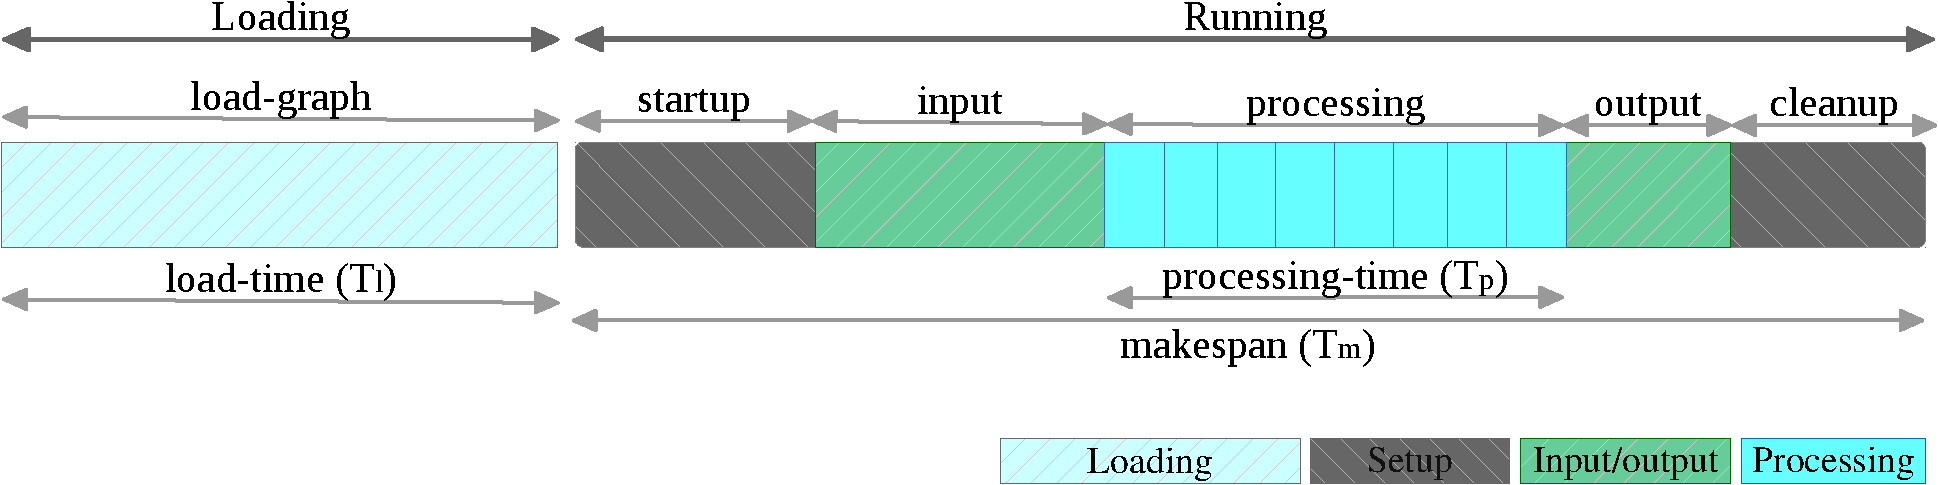
\includegraphics[width=0.9\linewidth]{figures/benchmark-job.pdf}
	\caption{A typical graph processing job with the underlying operations.}
	\label{fig:job}
\end{figure}


During the \textbf{Loading} step, the input graph data can be converted into an optimized system-specific data format and pre-loaded into a local/share/distributed storage system. Binary formats are allowed, however, the pre-processed data must be uniformly usable for any graph algorithms. \futureinversion{2.0}{I tried to clarify this but it's still quite vague. We should also include the word ``intermediate'' in the discussion (this is how the directory in the benchmark framework is called) [Gabor]}

During the \textbf{Running} step, the graph-processing system carries out a series of operations to facilitate efficient algorithm execution on the pre-processed data. These operations are categorized into three types: setup, input/output, and processing operations (see \fref{fig:job}).
\begin{itemize}
    \item \textbf{Setup operations} reserve computational resources in distributed environments, prepare the system for operation, clean up the environment after the termination of the job.
    \item \textbf{Input/output operations} transfer graph data from storage to the memory space, and convert the data to specific formats before/after data processing, and offload the outputs back to the storage. Some platforms load/unload data from a distributed file system, other distributed platforms from share/local storage in each node. \futureinversion{2.0}{Discuss that in-memory systems load the graph in this phase [Gabor]}
    \item \textbf{Processing operations} take in-memory data and process it according to an user-defined algorithm and its expression in a programming paradigm. Processing operations typically include iterative ``processing'' steps.
\end{itemize}








\subsection{Metrics} 
\label{sec:def:metrics}
This section describes the metrics used in Graphalytics. The Graphalytics benchmark includes several metrics to quantify the performance and other characteristics of the system under test. The performance of graph analytics systems is measured by the time spent on several phases in the execution of the benchmark. Graphalytics reports performance, throughput metrics, cost metrics, and ratio metrics, as follows.



The {\bf Performance metrics} report the execution time of various platform operations.

\begin{itemize}
	\item {\bf Load time} ($T_l$), in $\textit{seconds}$:  The time spent loading a particular graph into the system under test, including any preprocessing to convert the input graph to a format suitable for the system. This phase is executed once per graph before any commands are issued to execute specific algorithms.
	\item {\bf Makespan:} ($T_m$), in $\textit{seconds}$: The time between the Graphalytics driver issuing the command to execute an algorithm on a (previously uploaded) graph and the output of the algorithm being made available to the driver. The makespan can be further divided into processing time and overhead \futureinversion{2.0}{Define overhead [Gabor]}. The makespan metric corresponds to the operation of a {\it cold graph-processing system}, which depicts the situation where the system is started up, processes a single dataset using a single algorithm, and then is shut down.
	\item {\bf Processing time} ($T_p$), in $\textit{seconds}$: Time required to execute an actual algorithm. This does not include platform-specific overhead, such as allocating resources, loading the graph from the file system, or graph partitioning. The processing time metric corresponds to the operation of an in-production, {\it warmed-up graph-processing system}, where especially loading of the graph from the file system and graph partitioning, both of which are typically done only once and are algorithm-independent, are not considered.
\end{itemize}

The execution time is capped by the time-out duration configured in each benchmark. Once the time-out is reached, the graph-processing job is terminated, and the time-out duration is reported as the performance metrics instead.

The {\bf Throughput metrics} focus on the processing rate of the system under test. They use a notion of workload intensity, expressed in the graph-specific number of processed edges and vertices:
\begin{itemize}
	\item {\bf Edges Per Second} ($\textit{EPS}$), in $\textit{units} / \textit{second}$: The ratio between the number of edges processed (edge size) and the processing time ($T_p$) is used by other benchmarks (Graph500 in Table~\ref{tab:SummaryOfRelatedWorkAcronyms}) to quantify the rate of operation of the system under test. This is fine for edge-dominated algorithms, such as the BFS used in the same benchmarks, but does not explain the performance of vertex-dominated algorithms or of algorithms whose performance is a complex function of the structural properties of the dataset.
	
	\item {\bf Edges and Vertices per Second} ($\textit{EVPS}$), in $\textit{units} / \textit{second}$: Graphalytics uses the ratio between the sum of the number of edges and the number of vertices (graph size) processed by the system, and the processing time ($T_p$). EVPS is closely related to the scale of a graph, as defined by Graphalytics (see \sref{sec:definition_scale}).
\end{itemize}

Graphalytics also reports {\bf Cost metrics}:

\begin{itemize}
	\item {\bf Three-year Total Cost of Ownership} ($\textit{TCO}$), in $\textit{dollars}$: reported in compliance with the LDBC rules~\cite{ldbc_byelaws}, so {\it not} computed by Graphalytics. In particular, LDBC currently adapts the TPC standard pricing model v2.0.0~\cite{tpc_pricing}.
	
	\item {\bf Price-per-performance} ($\textit{PPP}$), in $\textit{dollars} / \textit{unit}$: as the ratio between TCO and EVPS. This is a metric included for compliance with the LDBC charter~\cite{ldbc_byelaws}.

	\futureinversion{2.0}{\item {\bf Three-year Total Energy Costs} ($\textit{TEC}$), in $\textit{watts}$: reported in compliance with the SPEC Power, so {\it not} computed by Graphalytics and {\it not} relying only on the metrics provided by the operating system software and hardware performance counters of current processors/systems.}
	
	\futureinversion{2.0}{\item {\bf Energy-per-performance} ($\textit{EPP}$), in $\textit{watts} / \textit{dollar}$: as the ratio between TEC and EVPS. This is a metric included for compliance with the LDBC charter~\cite{ldbc_byelaws}.}

\end{itemize}



\futureinversion{2.0}{
The {\bf Ratio metrics} reported by Graphalytics are:

\begin{itemize}
	\item {\bf Speedup}: The ratio between processing times for scaled and baseline resources. This metric is used to quantify the scalability of the system under test. %The baseline is defined as the minimum number of resources used in a particular experiment.
	The baseline is defined as the performance achieved by a reference graph-processing platform defined by the Graphalytics team until the next revision (here, the public version of Giraph with the reference drivers), in a reference environment defined by the Graphalytics team until the next revision (here, DAS5 in the Netherlands). The renewal process of Graphalytics (see \sref{sec:renewal}) can change the baseline.
\end{itemize}
}











\section{System Under Test} \label{sec:sut}

Responding to requirement R1 (see Section~\ref{sec:requirements}), the LDBC Graphalytics framework defines the System Under Test as the combined software platform and hardware environment that is able to execute graph-processing algorithms on graph datasets. This is an inclusive definition, and indeed Graphalytics has been executed in the lab of SUTs with software ranging from community-driven prototype systems, to vendor-optimized software; and with hardware ranging from beefy single-node multi-core systems, to single-node CPU and (multi-)GPU hybrid systems, to multi-node clusters with or without GPUs present. 

%%% POSSIBLE MODEL: from SPEC Cloud results
% https://www.spec.org/cloud_iaas2016/results/res2016q2/cloudiaas2016-20160404-00001.html#Instance Configuration
% cpu/mem/storage/net -> 10 items at sublevels
% \begin{verbatim}
%     Test
%       Line 2, indented
%       Line 2+, also indented as the previous
% \end{verbatim}

\section{Renewal Process} \label{sec:renewal}

To ensure the relevance of Graphalytics as a benchmark for future graph analytics systems, a renewal process is included in Graphalytics. This renewal process updates the workload of the benchmark to keep it relevant for increasingly powerful systems and developments in the graph analytics community. This results in a benchmark which is future-proof. Renewing the benchmark means renewing the algorithms as well as the datasets. For every new version of Graphalytics, a two-stage selection process will be used by the LDBC Graphalytics Task Force. The same selection process was used to derive the workload in the current version of the Graphalytics benchmark.

To achieve both workload representativeness and workload coverage, a two-stage selection process is used. \futureinversion{2.0}{This piece of text is repetitive [Gabor]} The first stage identifies classes of algorithms and datasets that are representative for real-world usage of graph analytics systems. In the second stage, algorithms and datasets are selected from the most common classes such that the resulting selection is diverse, i.e., the algorithms cover a variety of computation and communication patterns, and the datasets cover a range of sizes and a variety of graph characteristics.

Updated versions of the Graphalytics benchmark will also include renewed definitions of the scale classes defined in Section~\ref{sec:definition_scale}. The definition of the scale classes is derived from the capabilities of state-of-the-art graph analytics systems and common-off-the-shelf machines, which are expected to be improved over time. Thus, graphs that are considered to be large as of the publication of the first edition of Graphalytics (labeled $L'16$ to indicate the $2016$ edition) may be considered medium-sized graphs in the next edition (e.g., $M'20$).

